\documentclass[review]{elsarticle}

\usepackage[brazilian]{babel}
\usepackage[utf8]{inputenc}
\usepackage[T1]{fontenc}

\usepackage{lineno,hyperref}
\modulolinenumbers[5]

\usepackage{graphicx}
\graphicspath{ {./images/} }

%%%%%%%%%%%%%%%%%%%%%%%
%% Elsevier bibliography styles
%%%%%%%%%%%%%%%%%%%%%%%
%% To change the style, put a % in front of the second line of the current style and
%% remove the % from the second line of the style you would like to use.
%%%%%%%%%%%%%%%%%%%%%%%

%% Numbered
%\bibliographystyle{model1-num-names}

%% Numbered without titles
%\bibliographystyle{model1a-num-names}

%% Harvard
%\bibliographystyle{model2-names.bst}\biboptions{authoryear}

%% Vancouver numbered
%\usepackage{numcompress}\bibliographystyle{model3-num-names}

%% Vancouver name/year
%\usepackage{numcompress}\bibliographystyle{model4-names}\biboptions{authoryear}

%% APA style
%\bibliographystyle{model5-names}\biboptions{authoryear}

%% AMA style
%\usepackage{numcompress}\bibliographystyle{model6-num-names}

%% `Elsevier LaTeX' style
\bibliographystyle{elsarticle-num}
%%%%%%%%%%%%%%%%%%%%%%%

\begin{document}

\begin{frontmatter}

\title{Proposta de Projeto}

%% Authors
\author{Alexsandro Carvalho}
\ead{avsc@cin.ufpe.br}

\author{Jeffson Simões}
\ead{jcss3@cin.ufpe.br}

\begin{abstract}
Este texto é um relatório das atividades desenvolvidas no trabalho previamente proposto para a cadeira de Introdução à Ciência dos Dados do Centro de Informática - UFPE.
\end{abstract}

\begin{keyword}
data science\sep tourism
\end{keyword}

\end{frontmatter}

\linenumbers

\section{Introdução}
Nosso grupo decidiu analisar a influência dos diversos empreendimentos turísticos existentes no Brasil sobre a quantidade de turistas estrangeiros que visitam nosso país. Este texto vem relatar os resultados da nossa análise.

\section{Os Dados}
Originalmente, pretendíamos utilizar os datasets disponibilizados no Portal Brasileiro de Dados Abertos (abreviado no resto deste artigo como PBDA). Porém apenas os dados das hospedagens foram obtidos do mesmo.

Durante o desenvolvimento do projeto, encontramos uma ferramenta do Ministério do Turismo, o Extrator de Chegadas de Turistas Internacionais ao Brasil. Foi dado preferência a usá-lo no lugar do PBDA por 2 motivos: primeiro, porque ele estava mais atualizado e continha os dados de 2017; o segundo motivo foi porque os csvs do PBDA não mantinham um padrão nas suas colunas, o que dificultava juntar os dados.

\section{Análise Exploratória}

Para entender melhor os dados a serem trabalhados, foram feitos diversos gráficos com o objetivo de revelar fenômenos dos datasets que levassem a hipóteses interessantes de se analisar.

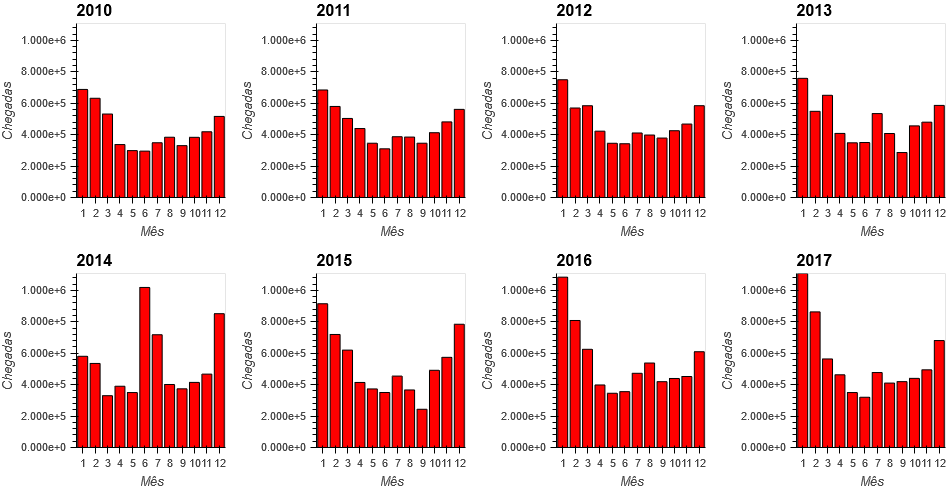
\includegraphics[width=\textwidth]{Bars-Year}

Inicialmente, foram feitos gráficos de barras do total de cada mês nos 8 últimos anos. Nesses gráficos, geralmente houve um padrão de o número de visitantes ser mais alto nos primeiros e últimos meses. Porém uma notável exceção foi o ano de 2014, onde os meses com maior número de turistas foram junho e julho, os meses durante os quais estava ocorrendo a Copa do Mundo. Isso serviu de motivação para analisar a hipótese do efeito de eventos esportivos no turismo.

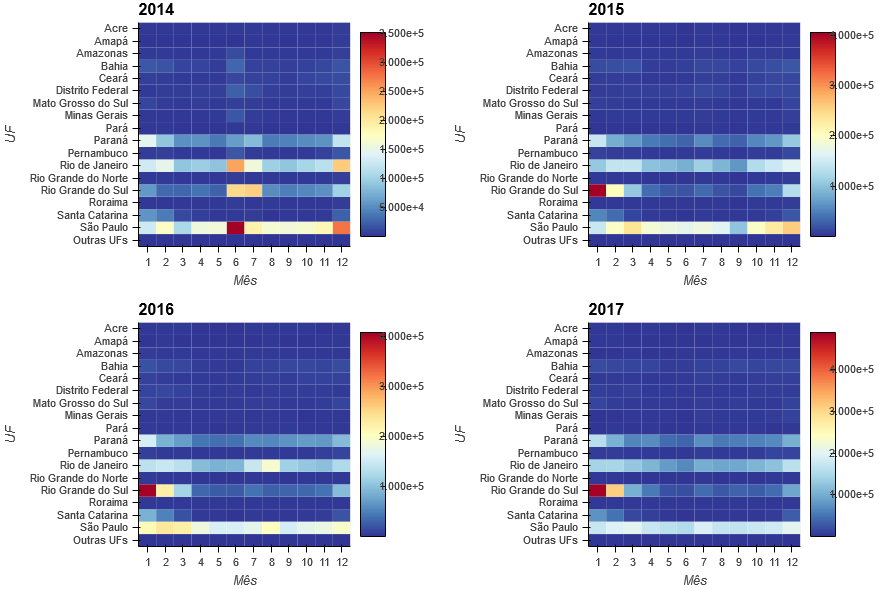
\includegraphics[width=\textwidth]{Heatmap-Year-UF}

Uma nova visualização, agora exibindo as chegadas mensais por estado. Com isso, foi observado que 4 estados concentram quase todos os turistas: Paraná, Rio de Janeiro, Rio Grande do Sul e São Paulo.

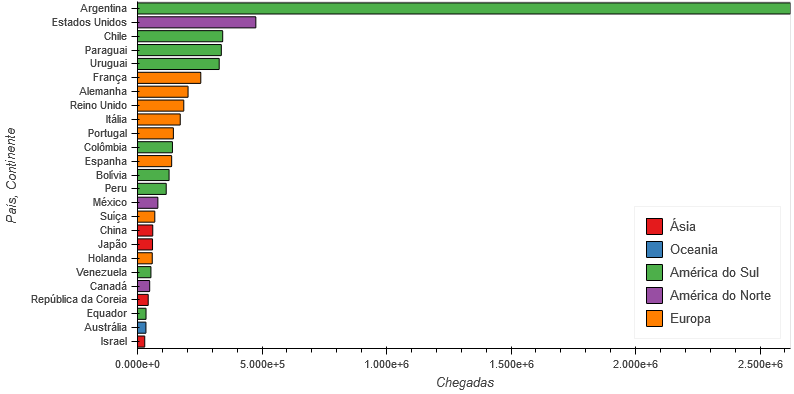
\includegraphics[width=\textwidth]{Bars-Country}

Uma plotagem dos 25 países com mais turistas visitando o Brasil. Nela é possível ver que o turistas argentinos são a grande maioria dos turistas estrangeiros. Além da Argentina, os países que mais visitam o Brasil são Sulamericanos ou europeus, com os EUA sendo a única exceção.

\section{Hipóteses testadas}
\subsection{Eventos esportivos afetam a chegada de turistas}
Para avaliar a hipótese de que os eventos esportivos Copa do Mundo e Olimpíadas afetaram a chegada de turistas no Brasil, foi feita uma regressão nos anos e meses, usando o histórico de 2008 a 2017. Para incluir os eventos na regressão, foram adicionadas uma variável para cada evento, indicando se ele estava ocorrendo no momento ou não.

Devido ao fato de os meses terem demonstrado uma influência não linear na chegada de turistas, também foi incluída na fórmula o quadrado do mês, pois assim a fórmula se tornaria uma equação do 2º grau, que possui o comportamento de crescer nas extremidades para cima ou para baixo, dependendo da concavidade.

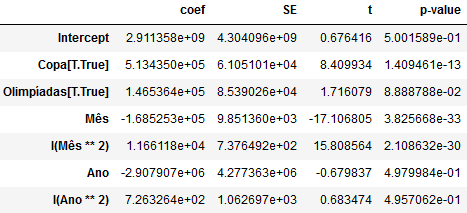
\includegraphics[width=\textwidth]{Regression-BR}

Os valores gerados acima mostram que a Copa do Mundo tem de fato efeito significativo (devido ao p-value baixo) e positivo, tendo atraído cerca de 500 mil turistas ao Brasil.

As Olimpíadas, por outro lado, tiveram um desempenho menor, e o p-value alto associado ao evento demonstra que ela não teve impacto significativo no número de turistas no Brasil. Porém, diferentemente da Copa do Mundo, as Olimpíadas foram um evento mais concentrado, ocorrendo apenas no Rio de Janeiro, sendo assim, foi feita uma nova regressão, porém com os turistas do Rio de Janeiro.

Analisando as outras variáveis da regressão, é possivel observar que o ano teve um p-value mais alto que o das Olimpíadas, indicando que ele é ainda menos influente que o evento. Isso pode ser um sinal de que o turismo brasileiro não possui crescimento anual, o que será investigado na próxima hipótese.

Já o mês, demonstrou o comportamento esperado. Como I(Mês ** 2) possui coeficiênte positivo, isso indica que a concavidade do gráfico está para cima, como observado na análise exploratória.

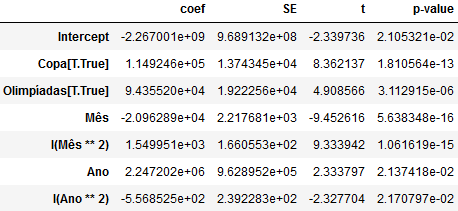
\includegraphics[width=\textwidth]{Regression-RJ}

Na segunda regressão, restrita ao Rio de Janeiro, as Olimpíadas tiveram um p-value bem menor, e seu coeficiente se aproximou do da Copa do Mundo. Isso mostra que a localidade das Olimpíadas fez com que o efeito delas também fosse local.

A conclusão geral dessa hipótese é a de que os eventos esportivos impulsionam o turismo, porém a abrangência desse impulso é limitada aos locais onde o evento está ocorrendo.

\subsection{O turismo no Brasil não está crescendo}
Para avaliar essa hipótese, foi plotado um gráfico contendo a média de turistas pra cada ano de 2008 a 2017.

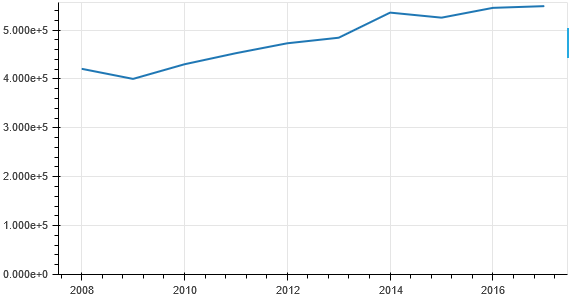
\includegraphics[width=\textwidth]{Segment-Tourist-Year}

O gráfico demonstrou que houve aumento, o que a princípio, parece contradizer a hipótese. Para entender melhor a situação, foi plotado um segundo gráfico mais granularizado, que contém o total de turistas por mês.

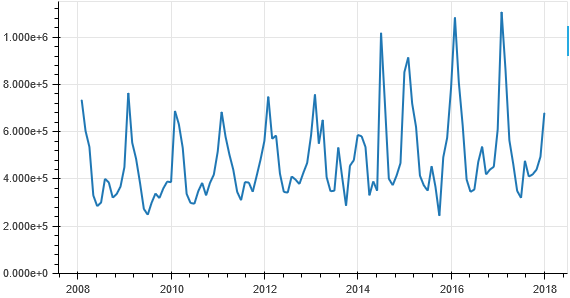
\includegraphics[width=\textwidth]{Segment-Tourist-Month}

O segundo gráfico mostra o porquê do ano não demonstrar influência na chegada pela regressão. As oscilações causadas pelo efeito dos meses são tão grandes que elas mascaram o crescimento anual do número de turistas. A conclusão aqui é a de que o turismo está de fato crescendo com os anos, mas pouco.

\subsection{As Hospedagens, que oferecem X idioma no atendimento a Turistas estrangeiros, influênciam no fluxo de Turistas}

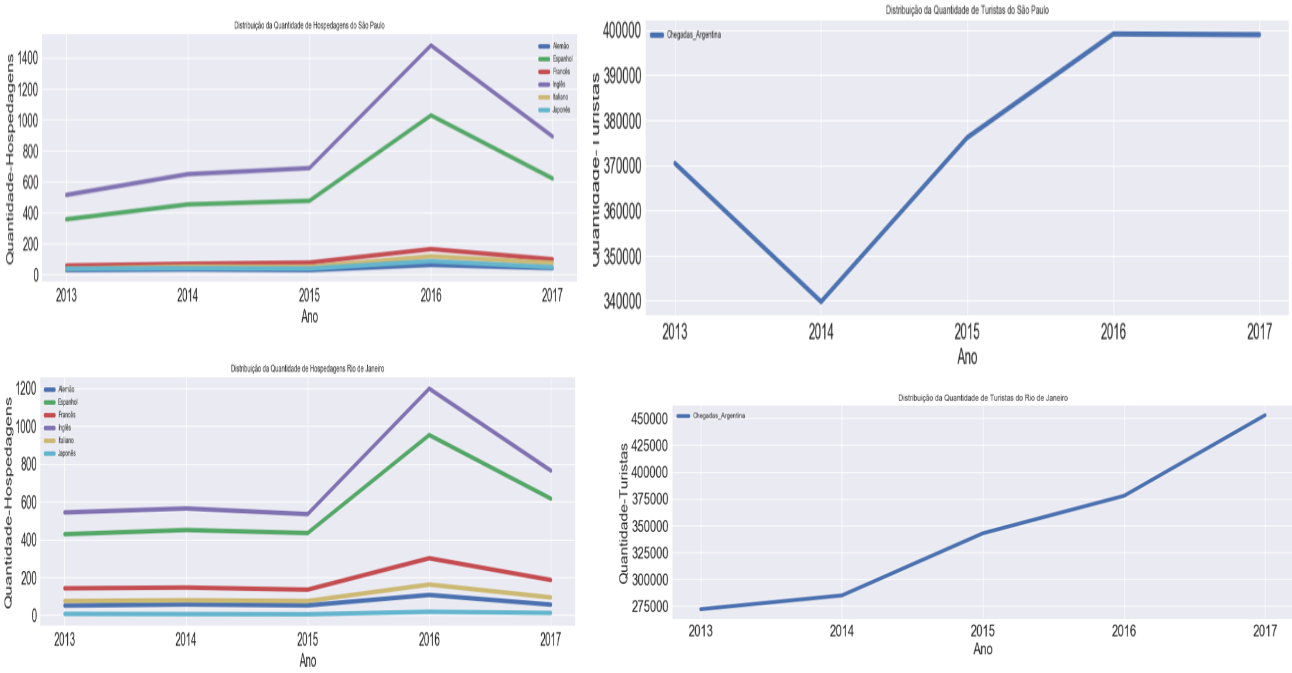
\includegraphics[width=\textwidth]{Segment-Host-Tourist}
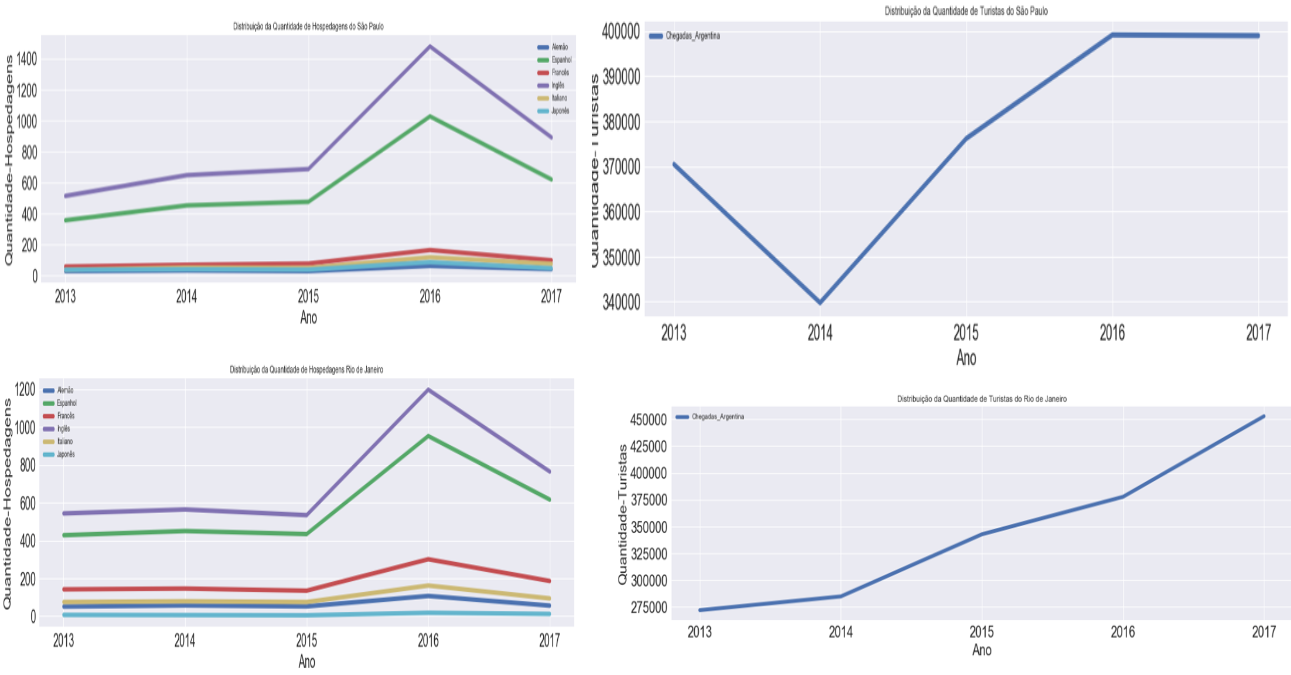
\includegraphics[width=\textwidth]{Segment-Host-Tourist-2}

Para avaliar as hipóteses, criamos gráficos das séries temporais obtidas - Chegadas de Turistas e Quantidade de Hospedagens - e comparamos as variáveis nos dois gráficos de acordo com o intervalo de tempo, no caso, comparamos a quantidade de hospedagens que ofereciam atendimento em espanhol com a série temporal da quantidade de turistas argentinos que chegavam.

Devido a encontrarmos um pico na quantidade de hospedagens no ano de 2016 pudemos ver que as Olimpíadas influenciaram na quantidade de hospedagens.

\section{Conclusão}
Analisando os dados pudemos entender um pouco sobre a situação do turismo brasileiro, quem nos visita, quando somos visitados, para onde esses turistas vão, e saber o que os atrai e o que não os atrai para cá.

\end{document}